\documentclass{homework}
\title{Homework 2}
\begin{document}
\maketitle

\begin{problem}
We use \(\boxed x\) to denote the closest
floating-point representation of \(x\). Then
by definition we have
\[\frac{\left|\boxed{x} - x\right|}{x} \le \epsilon\]
where \(\epsilon\) is the machine precision.
We use \(\epsilon_k\) for arbitrary constants within
machine precision.

For addition, given any two real numbers \(x,y\),
\[\begin{aligned}
  \boxed{\boxed x + \boxed y}
&= \boxed{x(1+\epsilon_1) + y(1+\epsilon_2)}\\
&= \left[x(1 + \epsilon_1) + y(1 + \epsilon_2)\right](1+\epsilon_3)\\
&= x(1 + \epsilon_1 + \epsilon_3 + \epsilon_1\epsilon_3)
+ y(1 + \epsilon_2 + \epsilon_3 + \epsilon_2\epsilon_3).
\end{aligned}\]
Let \(\tilde x, \tilde y\) be the two terms, respectively.
Then the floating-point addition of \(x\) and \(y\)
is equal to \(\tilde x + \tilde y\), both of which
has relative error less than \(3\epsilon = O(\epsilon)\).
For subtraction the analysis is the same apart from
sign differences. For multiplication
\[\begin{aligned}
  \boxed{\boxed x \cdot \boxed y}
&= \boxed{xy(1+\epsilon_1)(1+\epsilon_2)}\\
&= xy(1+\epsilon_1)(1+\epsilon_2)(1+\epsilon_3)\\
&= xy(1 + O(\epsilon)),
\end{aligned}\]
so we can take \(\tilde x = x, \tilde y =
y(1+\epsilon_1)(1+\epsilon_2)(1+\epsilon_3)\).
For division the same calculation leads to
\[\frac{x(1+\epsilon_1)}{y(1+\epsilon_2)}(1+\epsilon_3).\]
And since we also have
\(\frac{(1+\epsilon_1)}{(1+\epsilon_2)}(1+\epsilon_3) = 1+O(\epsilon),\)
division is backwards stable.
\end{problem}

\begin{problem}\(\)\par
\begin{enumerate}[label=(\roman*)]
\item Take \[\hat f(x) = f(x)[1+\epsilon g(x)]\]
where \(|g(x)| \le 1\) is a fixed perturbation.
By definition we have
\[\begin{aligned}
\kappa(h) &= \limsup_{\epsilon \to 0^+}
\left|\frac{\hat f(x+h) - \hat f(x)}{h} - \frac{f(x+h)-f(x)}{h}\right|
\cdot \frac{1}{\epsilon}\\
&= \limsup_{\epsilon \to 0^+}
\left|\frac{f(x+h)g(x+h) - f(x)g(x)}h\right|\\
&= f(x)g'(x) + f'(x)g(x) + O(h).
\end{aligned}\]
\item The error should first decrease
quadratically, since Taylor expanding
we have \[\frac{e^{1 + h} - e^{1-h}}{2h}
= e\frac{h + \frac{h^2}{2} + h - \frac{h^2}{2} + O(h^3)}{2h}
= e(1 + O(h^2)).\]
At smaller \(h\), the error should increase again
since \((1 + h) - (1 - h)\) will start to deviate
from \(2h\) because of machine precision. It will
gradually increase until the error reaches \(e\),
i.e. when the derivative is evaluated to be \(0\).
\end{enumerate}
\begin{matlab}
hs = 2 .^ (-1:-1:-60);
ds = (exp(1+hs) - exp(1-hs)) ./ (2 * hs);
d = exp(1);

figure(1);
loglog(hs, abs(ds - d));
\end{matlab}
\begin{center}
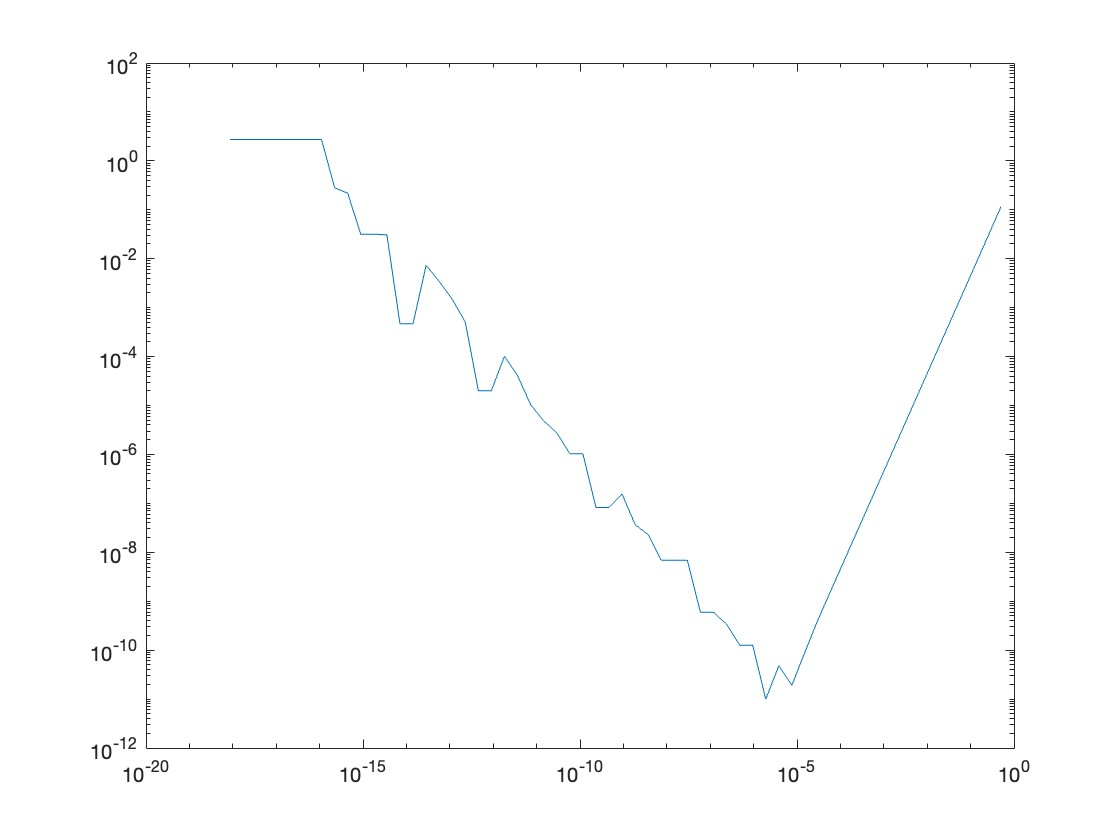
\includegraphics[width=0.7\textwidth]{Hw2-Fig1.jpg}
\end{center}
This agrees with the prediction.
\end{problem}

\begin{problem}
Recall that the basis functions are
\[\ell_j(x) = \prod_{i \ne j} \frac{x - x_i}{x_j - x_m}.\]

\begin{enumerate}[label=(\roman*)]
\item Each basis function satisfies
\[\ell_i(x_j) = \begin{cases}
  1 & i = j\\
  0 & i\ne j.
\end{cases}\]
Therefore the sum \(f = \sum_k \ell_k\) satisfies
\(f(x_j) = 1\). But since \((f - 1)\) is a polynomial
of degree at most \(n\), and it has at least
\((n+1)\) roots, therefore it must be
identically zero. This proves that
\(f = \sum_k \ell_k = 1\).

\item By the exact same analysis, we know that
\(f = \sum_k x_k^j \ell_k\) agrees with \(x^j\)
at \(x_0,\dots,x_n\), therefore \(f(x) - x^j\)
is a polynomial with at least \((n+1)\) roots.
Since \(j \le n\), the overall degree is still
no more than \(n\), and therefore \(f(x) = x^j\)
identically.

\item We expand using the previous two results
and the binomial theorem:
\[\begin{aligned}
\sum_{k=0}^n (x_k - x)^j \ell_k(x)
&= \sum_{k=0}^n \underbrace{\sum_{i = 0}^j
  \binom{j}{i} (-x)^i x_k^{j-i}}_{\text{binomial theorem}} \ell_k(x)\\
&= \sum_{i = 0}^j \binom{j}{i} (-x)^i
  \underbrace{\sum_{k=0}^n x_k^{j-i} \ell_k(x)}_{\text{(ii)}}\\
&= \underbrace{\sum_{i = 0}^j \binom{j}{i} (-x)^i \cdot x^{j-i}}_{\text{binomial theorem}}\\
&= (x - x)^j = 0.
\end{aligned}\]

\item Using the product derivative rule
\[w'(x) = \sum_{j = 0}^n
\prod_{k \ne j} (x - x_k).\]
Substituting \(x = x_k\), all but one factor vanishes,
and therefore the quotient
\[\frac{w(x)}{w'(x_k)}
= \frac{\prod_{j=0}^n (x - x_j)}{\prod_{j\ne k} (x_k - x_j)}.\]
Further divided by \((x - x_k)\), this gives
the desired result.\qed
\end{enumerate}
\renewcommand{\qed}{}
\end{problem}

\begin{problem}
We define the Lagrange interpolation for a set of
points, and define a helper function to interpolate
from the data of a given function:
\begin{matlab}
function val = lagrange(Xs, Ys, x)
    n = length(Xs);
    val = 0;
    for i = 1:n
        factors = (x - Xs) ./ (Xs(i) - Xs);
        factors(i) = [];
        val = val + Ys(i) * prod(factors);
    end
end

function val = interpolate(f, Xs, x)
    val = lagrange(Xs, arrayfun(f, Xs), x);
end
\end{matlab}
To graph these functions we need to set the \(x\)-coordinates
to evaluate them. Since we are interested in the
interpolating performance, we evaluate in the
interval \([-1,1]\). We also define the function
to be interpolated by a function handle:
\begin{matlab}
pts = (-1:0.01:1);
f = @(x) 1/(1+25*x^2);
\end{matlab}
Now we do the graphing.
\begin{matlab}
figure(2);
hold on
for N = [10 25 50 80 100]
    nodes = (0:N) * 2 / N - 1;
    ylim([-2 2]);

    plot(pts, arrayfun(@(x) interpolate(f, nodes, x) - f(x), pts), "DisplayName", "N = " + string(N))
end
hold off
\end{matlab}
This produces the following graphs.

\begin{center}
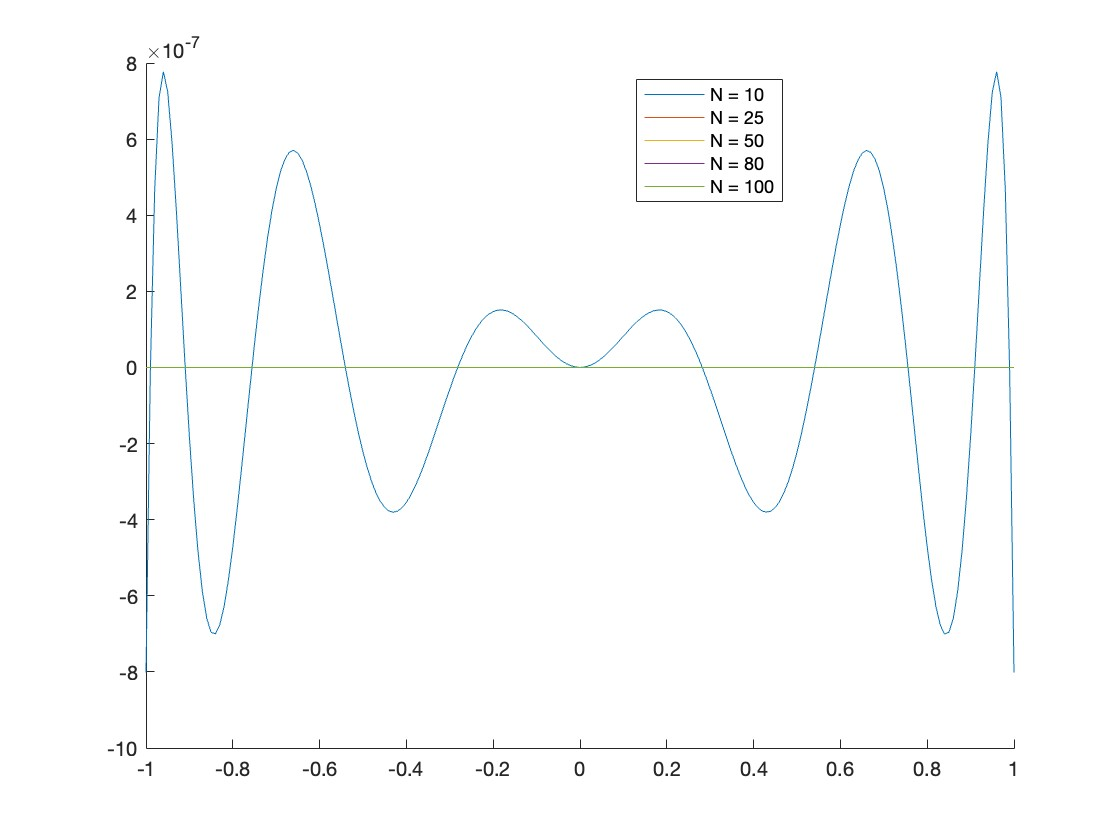
\includegraphics[width=0.4\textwidth]{Hw2-Fig2-Gauss-Chebyshev.jpg}
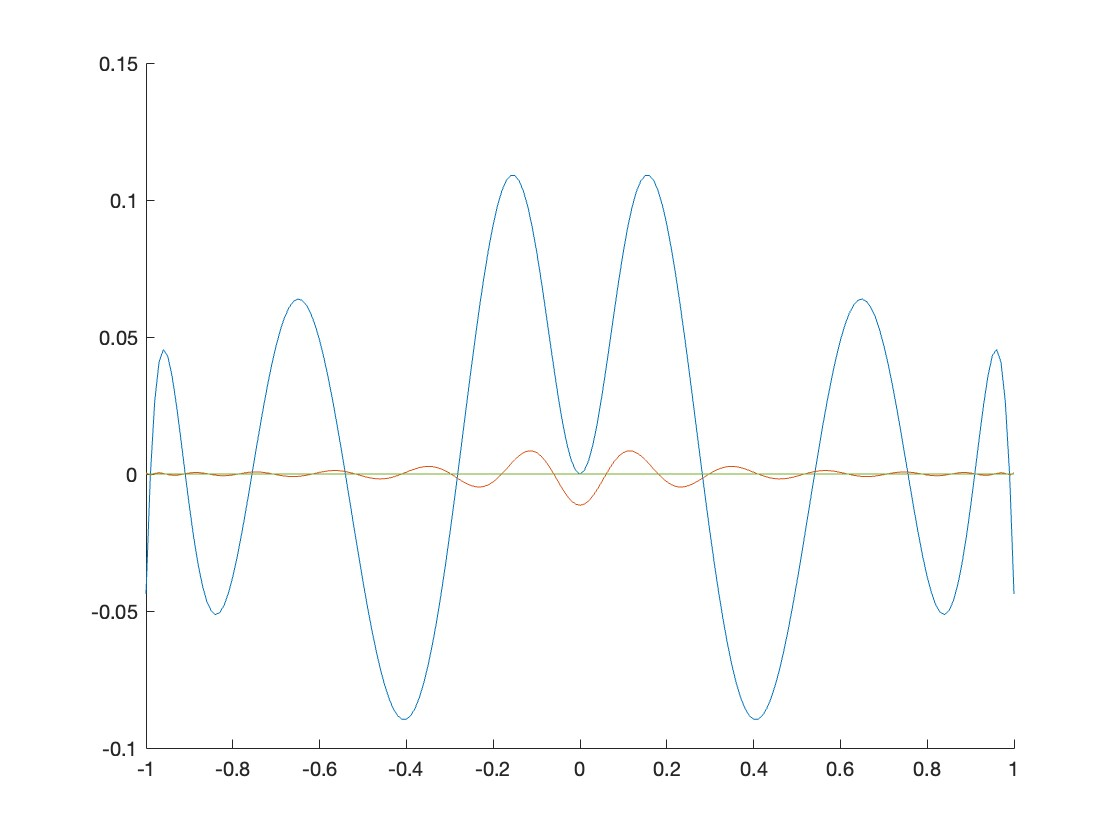
\includegraphics[width=0.4\textwidth]{Hw2-Fig2-Hat-Chebyshev.jpg}\\
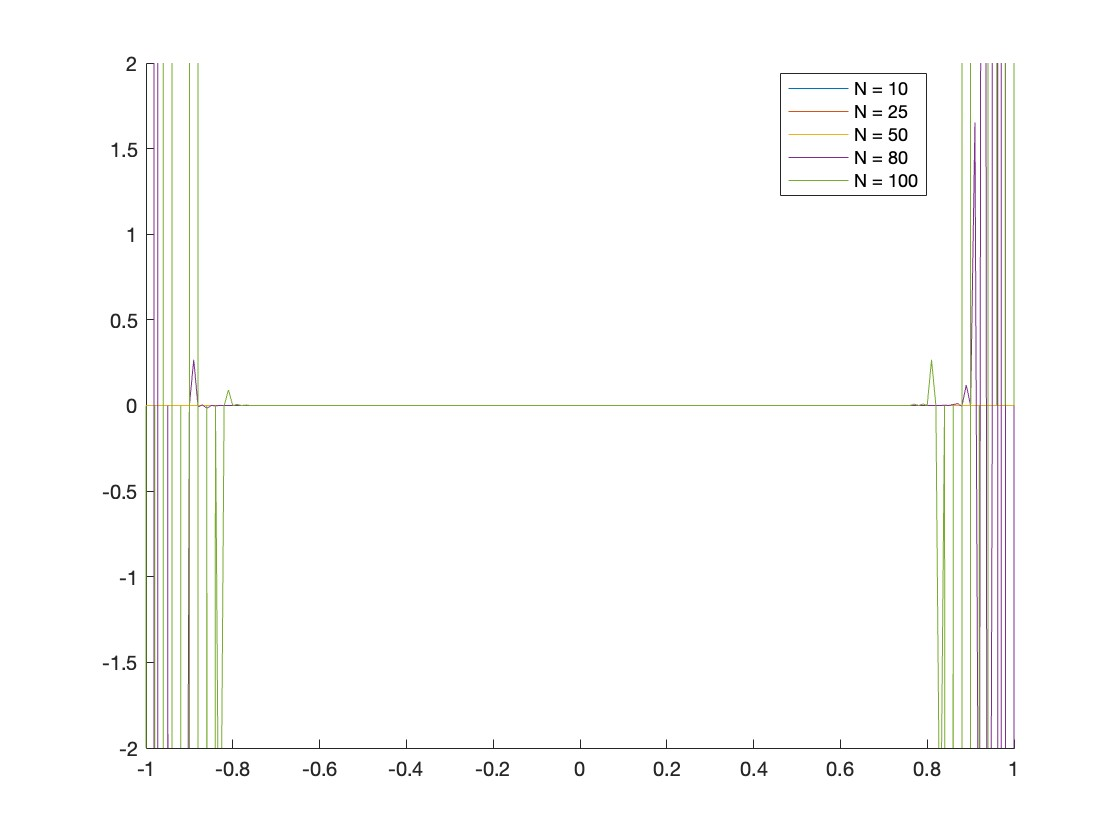
\includegraphics[width=0.4\textwidth]{Hw2-Fig2-Gauss-Equidistant.jpg}
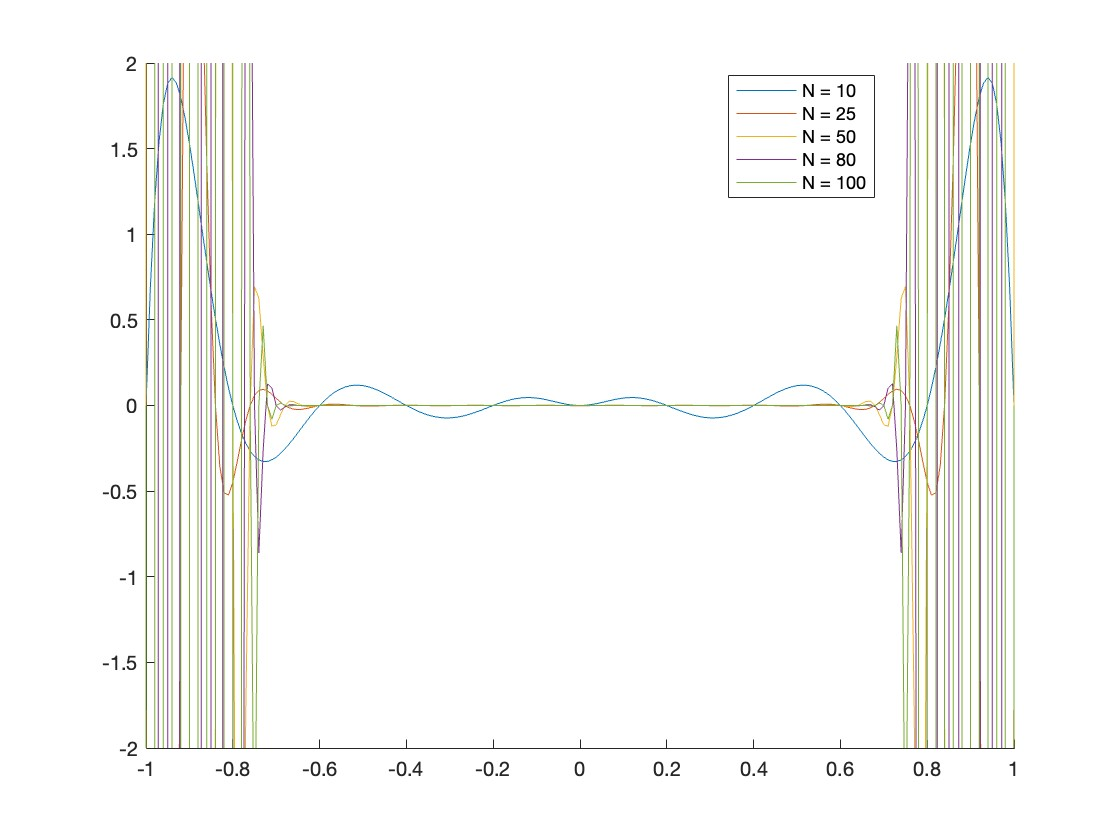
\includegraphics[width=0.4\textwidth]{Hw2-Fig2-Hat-Equidistant.jpg}\\
\end{center}
The left two graphs are for the Gauss
function; the upper two uses Chebyshev nodes; vice versa
for the right and the lower ones. For the Chebyshev
nodes, the polynomial quickly converges to the
desired function uniformly. For the equidistant
nodes the convergence is faster in the center region,
but the error quickly goes out of bounds at the edge.

Repeatedly integrating by parts, we can arrive
at the error estimate
\[|f(x) - P(x)| \le \frac{\prod_{k=0}^n (x - x_k)}{(n+1)!}
\sup_{x_0 \le x \le x_n} |f^{(n+1)}(x)|.\]
Let's first look at the \(f^{(n+1)}(x)\) factor.
For the Gaussian function
\[\frac{1}{n!}\frac{\d[^n]}{\d[x^n]}e^{-x^2} \le 1\]
is a well-known bound. But for
\(\frac{1}{1+25x^2}\) the supremum is at least \(5^n\),
which grows without bound. As for the
\(\prod_k (x - x_k)\) factor, for equidistant
nodes this factor is unbounded, while
the Chebyshev nodes minimizes the supremum
at \(2^{-n}\).

Combining this we see that the Chebyshev
nodes have much better convergence properties
than equidistant nodes, and the interpolation of
\(\frac{1}{1+25x^2}\) converges much more slowly.
This does not give an intuitive explanation why
equidistant interpolation \emph{does} have the
Runge phenomenon in this particular case, only
a justification that this \emph{can} happen.
\end{problem}

\newpage
\section*{Appendix: Source Code}
\matlabfile{Hw2.m}

\end{document}
